% ---------
%  Compile with "pdflatex hw0".
% --------
%!TEX TS-program = pdflatex
%!TEX encoding = UTF-8 Unicode

\documentclass[11pt]{article}
\usepackage{jeffe,handout,graphicx}
\usepackage[utf8]{inputenc}		% Allow some non-ASCII Unicode in source

% =========================================================
%   Define common stuff for solution headers
% =========================================================
\pagenumbering{arabic}
\Class{ECE 198}
\Semester{Fall 2019}
\Authors{1}
\AuthorOne{Jin Yucheng}{yucheng9}
%\AuthorTwo{Friday Caliban}{fcaliban}
%\AuthorThree{Duncan Quagmire}{dquagmir}
%\Section{}
\usepackage{float}

% =========================================================
\begin{document}

% ---------------------------------------------------------


\HomeworkHeader{4}{1-4}	% homework number, problem number

\begin{solution}
%These are, without exception, inappropriate inquiries, a phrase which here means “all the wrong questions”.  Here are the questions you should have asked instead:
%\begin{enumerate}[(a)]
%\item Why would someone say something was stolen when it was never theirs to begin with?
%\item How could someone who was missing be in two places at once?
%\item Why would someone destroy one building when they really wanted to destroy another?
%\end{enumerate}
%\begin{enumerate} [(a)]

\item (1) Prove that the iterative program for finding $F_{n}$ given in Section 5.4 is correct: Fib($x$): if $x$ = 0, return 0; if $x$ = 1, return 1; else, return Fib($x-1$) + Fib($x-2$).
 \item
\noindent\fbox{
    \parbox{\textwidth}{
\item
\begin{itemize}
\item Basis Step: when $x$ = 0, Fib(0) successfully returns 0 and when $x$ = 1, Fib(1) successfully returns 1, Fib($x$) is correct when $x$ = 0 or 1.
\item Inductive Step: Assume for non-negative integers $k$ and $n$ ($n \geq 2$), for each $k$, such that $k \leq n$, Fib($k$) is correct. Therefore, Fib($n+1$) will return Fib($n$) + Fib($n-1$), by the inductive hypothesis, Fib($n$) and Fib($n-1$) correctly compute $F_{n}$ and $F_{n-1}$, therefore, Fib($n+1$) correctly computes $F_{n+1}$.
\end{itemize}
So the iterative program for finding $F_{n}$ given in Section 5.4 is correct.
    }
}
\item
\item (2) Find the chromatic number of the graph below and prove your result with two-way bounding
\begin{figure}[H]
\centering
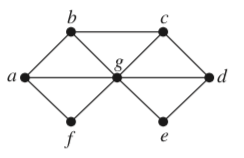
\includegraphics [width = 6cm]{Screen.png}
\item
\end{figure}
 \item
\noindent\fbox{
    \parbox{\textwidth}{
\item
The chromatic number of the above graph is 3.
\begin{itemize}
\item The chromatic number $\leq$ 3: since if we assign red to $g$, green to $b, d, f$, and blue to $a, c, e$, then no adjacent vertices have the same color, so the chromatic number is at most 3.
\item The chromatic number $\geq$ 3: since $b$ is adjacent to $g$, $b$ and $g$ must have different colors; $g$ is adjacent to $a$, $a$ and $g$ must have different colors; $a$ is adjacent to $b$, $a$ and $b$ must have different colors. Therefore, $a, b, g$ all have different colors pairwisely, then the chromatic number is at least 3.
\end{itemize}
  }
}
\pagebreak
\\
(3) Let $G_{1}$ and $G_{2}$ be CFGs with languages $L(G_{1})$ and $L(G_{2})$ respectively. Prove there exists a CFG with language $L(G_{1}) \cup L(G_{2})$.
 \item 
\noindent\fbox{
    \parbox{\textwidth}{
\item
Denote language $L(G_{1})$ generated by CFG $G_{1}$ as \{$V_{1}, T_{1}, S_{1}, P_{1}$\}, language $L(G_{2})$ generated by CFG $G_{2}$ as \{$V_{2}, T_{2}, S_{2}, P_{2}$\}. Denote $G$ as \{$V, T, S, P$\}, where,
\begin{itemize}
\item $V = V_{1} \cup V_{2} \cup S$, where $S$ denotes the new start symbol.
\item $T = T_{1} \cup T_{2}$.
\item $S$ is the new start symbol.
\item $P = P_{1} \cup P_{2} \cup \{S \rightarrow S_{1}, S \rightarrow S_{2}\}$.
\end{itemize}
Then $L(G)$ is the union of $L(G_{1})$ and $L(G_{2})$, therefore, there exists a CFG $G$ with $L(G) = L(G_{1}) \cup L(G_{2})$.

    }
}
\item
\item (4) Prove that if FSM $A$ accepts language $L_{a}$ and FSM $B$ accepts language $L_{b}$, there exists a FSM that accepts language $L_{c}$ = \{$xy$ | $x \in L_{a}$ and $y \in L_{b}$\} by constructing that FSM and using two-way bounding to show that your FSM accepts exactly $L_{c}$.
 \item
\noindent\fbox{
    \parbox{\textwidth}{
\item  
Denote FSM $A$ as \{$S_{a}, I_{a}, O_{a}, f_{a}, g_{a}, s_{0, a}$\}, FSM $B$ as \{$S_{b}, I_{b}, O_{b}, f_{b}, g_{b}, s_{0, b}$\}. \\
Denote FSM $C$ as \{$S_{c}, I_{c}, O_{c}, f_{c}, g_{c}, s_{0, a}$\}, where,
\begin{itemize}
\item $S_{c} = S_{a} \cup S_{b}$.
\item $I_{c} = I_{a} \cup I_{b}$.
\item $O_{c} = O_{a} \cup O_{b}$.
\item $f_{c} = f_{a} \cup f_{b} \cup f_{new}$, where the states of $f_{new}$ are states $s_{i} \in S_{a}$, such that there exists an input $j$, and another state $s_{k} \in S_{a}$, that $f(s_{k}, j) = s_{i}$ and $g_{a}(s_{k}, j) = 1$; the inputs of $f_{new}$ are elements in $I_{b}$, denote $l$ as one element in $I_{b}$.  $g_{c} = g_{a'} \cup g_{b} \cup g_{new}$, where $g_{a'}$ assigns 0 for each state and input pair in FSM $A$. 
\\ $f_{new}(s_{i}, l) = f_{b}(s_{0, b}, l), g_{new}(s_{i}, l) = g_{b}(s_{0, b}, l)$ (actually $f_{c}$, is not a total function because there are some implicitly rejected states).
\item $s_{0, a}$ is the start state.
\end{itemize}
Then prove $C$ accepts exactly $L_{c}$.
\begin{itemize}
\item for every string $w = xy$ such that $x \in L_{a}$ and $y \in L_{b}$, since if $x \in L_{a}$, then the last output bit is 1, because all states $s_i \in S_{a}$ with a transition function $f(s_{k}, j) = s_{i}$ and  an output function $g_{a}(s_{k}, j) = 1$ is assigned $f_{new}(s_{i}, l) = f_{b}(s_{0, b}, l)$ for every input $l$ in $I_{b}$, so all strings accepted by $A$ with at least one input $l$ in $I_{b}$ can transit to $B$, and $B$ accepts all strings in $L_{b}$, therefore $C$ accepts every string $w = xy$  such that $x \in L_{a}$ and $y \in L_{b}$. 
\item for every string $w = xy$ such that $x \notin L_{a}$ or $y \notin L_{b}$, because if $x \notin L_{a}$, then $w$ is not accepted by $L_{a}$, and there is no transition function that can transit the state upto input string $xl$ ($l \in I_{b}$) to B; if $y \notin L_{b}$, then the last output digit must be 0, therefore $C$ rejects every string $w = xy$  such that $x \notin L_{a}$ or $y \notin L_{b}$. 
\end{itemize}

    }
}
\end{solution}

\end{document}